\section{Model Architecture}

This study proposes a modified SAGE framework named \textbf{FeatureSAGE}. The architecture combines a pretrained StyleGAN2 generator, the StyleFeatureEditor inverter and Feature Editor, and SAGE's attribute group editing mechanism. The purpose of the modification is to improve the inversion stage of SAGE by representing each input image with both a layer-wise latent code and an intermediate feature tensor. This design follows the observation of \citet{ding2023stableattributegroupediting} that stronger inversion can further improve the potential of SAGE for generative augmentation, and it follows \citet{bobkov2024devildetailsstylefeatureeditordetailrich} in using both $W^+$ latents and feature latents for detail-preserving editing.

The main components of FeatureSAGE are:

\begin{enumerate}
    \item \textbf{StyleGAN2 generator:} The pretrained StyleGAN2 generator synthesizes images from latent codes. In FeatureSAGE, the generator receives the edited $W^+$ latent code together with an edited intermediate feature tensor produced by the Feature Editor.
    
    \item \textbf{StyleFeatureEditor inverter:} The inverter replaces the original pSp inversion module used in SAGE. For each input image, it predicts a $W^+$ latent code and an intermediate feature tensor. The $W^+$ code captures layer-wise style information, while the feature tensor carries spatial details that are difficult to preserve using latent codes alone.

    \item \textbf{Feature Editor:} The Feature Editor modifies the extracted feature tensor according to the latent-space edit. This allows the decoder path of the generator to synthesize images whose semantic edit is controlled by the latent code while finer details are supported by feature-level information.

    \item \textbf{SAGE attribute group editing:} The attribute factorization, class embedding mapping, and adaptive editing blocks are retained from SAGE. These blocks estimate category-relevant embeddings and category-irrelevant directions so that unseen classes can be edited under a one-shot setting.
\end{enumerate}

% ======================================================================================================

\subsection{Framework Overview}

\newgeometry{
    top=1cm,
    bottom=1cm,
    left=1cm,
    right=1cm
}

\begin{landscape}
    \begin{figure}[p]
        \centering
        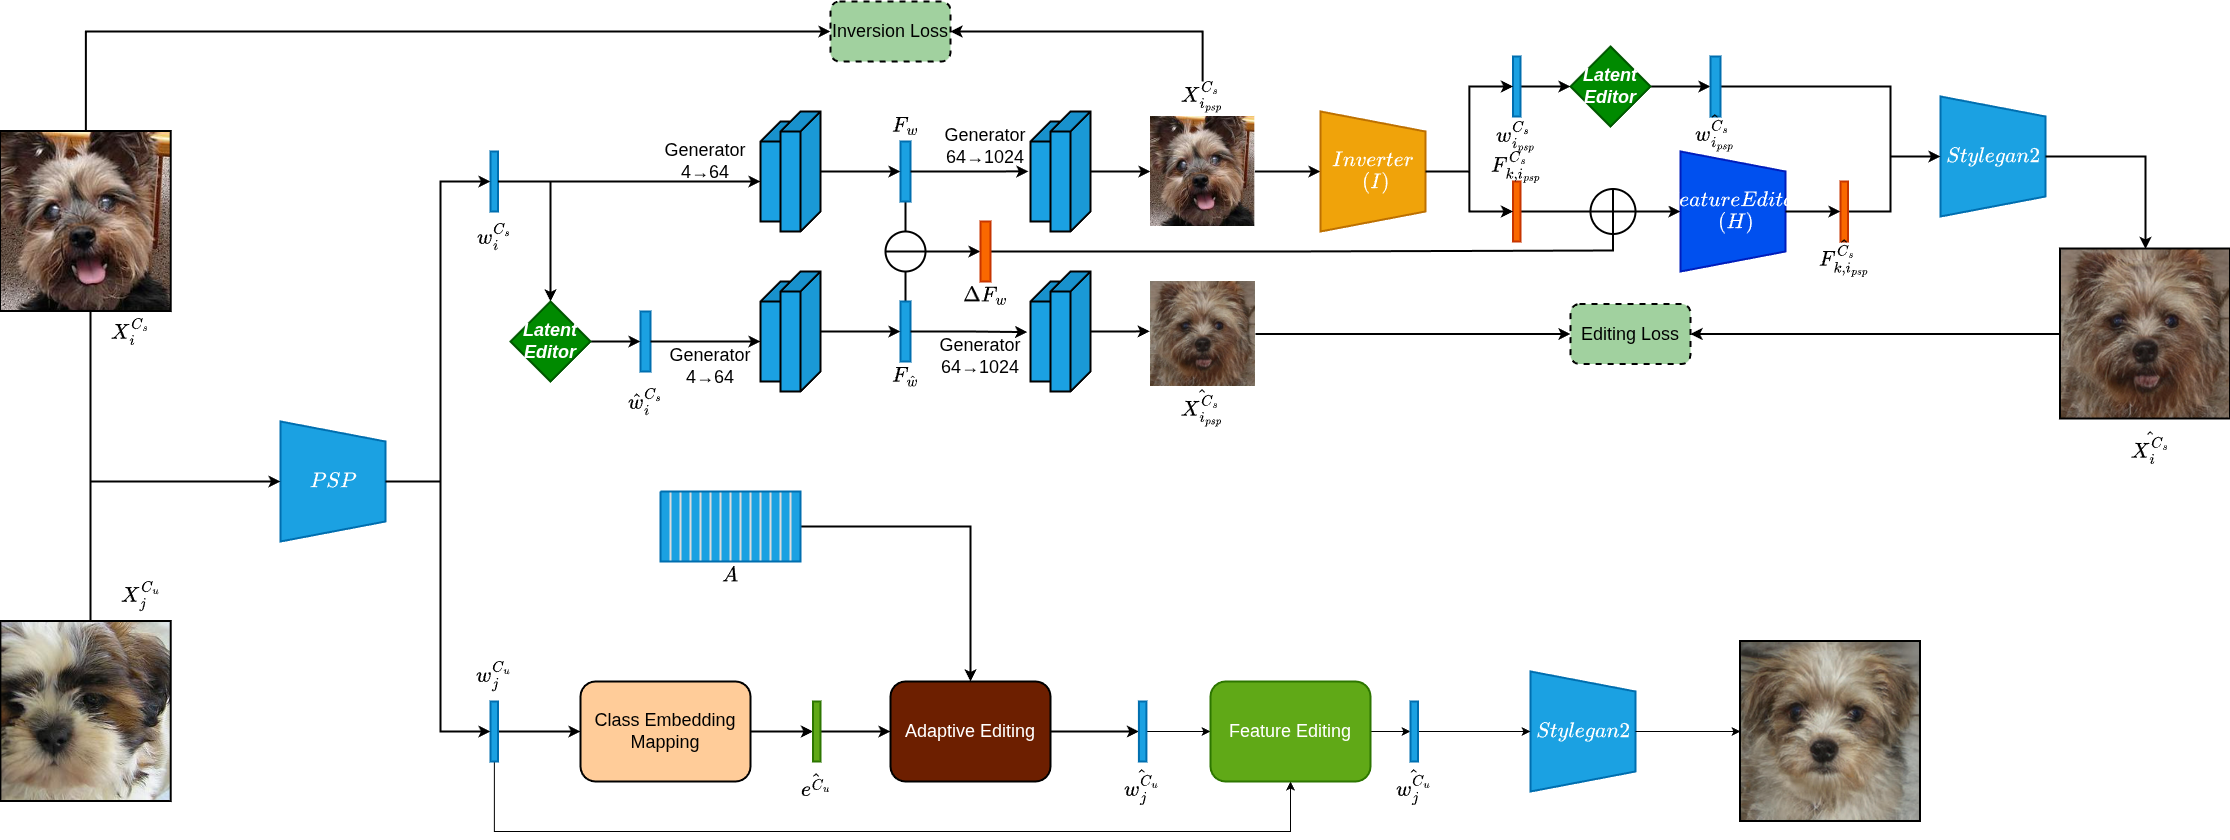
\includegraphics[
            width=\linewidth,
            height=\textheight,
            keepaspectratio
        ]{images/framework.png}
        \caption{FeatureSAGE framework}
        \label{fig:feature_sage_framework}
    \end{figure}
\end{landscape}

\restoregeometry

Figure~\ref{fig:feature_sage_framework} shows the overall FeatureSAGE framework. The training set for seen categories and the testing set for unseen categories are represented in Equation~\ref{eq:train-test-sets}:

\begin{equation}
D_{\mathrm{train}}=\{x_i^{C_s}\}_{i=1}^{N_s}, \qquad
D_{\mathrm{test}}=\{x_i^{C_u}\}_{i=1}^{N_u},
\label{eq:train-test-sets}
\end{equation}

where $x_i^{C_s}$ denotes an image from a seen category $C_s$, $x_i^{C_u}$ denotes an image from an unseen category $C_u$, and $N_s$ and $N_u$ denote the number of samples used from the seen and unseen splits, respectively. Equation~\ref{eq:train-test-sets} provides the notation used throughout the methodology for separating classes used in training from classes used during one-shot evaluation.

% ======================================================================================================

\subsection{Feature Extraction and Latent-Space Representation}

Feature extraction occurs before the generator synthesizes an output image. In the baseline SAGE configuration, the pSp encoder maps an input image into the extended StyleGAN2 latent space, as shown in Equation~\ref{eq:psp-inversion}:

\begin{equation}
PSP(x_i^{C_s}) = w_i^{C_s}, \qquad w_i^{C_s}\in W^+.
\label{eq:psp-inversion}
\end{equation}

In Equation~\ref{eq:psp-inversion}, $PSP(\cdot)$ is the pSp encoder and $w_i^{C_s}$ is the predicted $W^+$ latent code for a seen-category image. The $W^+$ space is important because it contains separate style vectors for the generator layers, allowing the model to represent coarse-to-fine visual attributes.

In FeatureSAGE, the StyleFeatureEditor inverter extracts two representations from an image, as defined in Equation~\ref{eq:sfe-inversion}:

\begin{equation}
I(x_i^{C}) = \left(w_i^{C}, F_{k,i}^{C}\right), \qquad
w_i^{C}\in W^+.
\label{eq:sfe-inversion}
\end{equation}

Here, $I(\cdot)$ is the StyleFeatureEditor inverter, $w_i^{C}$ is the layer-wise latent code, and $F_{k,i}^{C}$ is the intermediate feature tensor extracted at generator layer $k$. The document uses the ninth StyleGAN feature layer for feature injection. The latent code represents semantic and style-level information, while the feature tensor represents spatial detail and texture information. These two extracted features are significant because the latent code controls the edit direction, whereas the feature tensor helps preserve local details during synthesis.

The generator can also expose intermediate features for an original and edited latent code. Equation~\ref{eq:generator-feature-extraction} defines these generator-side features:

\begin{equation}
(x_{i,\mathrm{psp}}^{C_s},F_w)=G(w_i^{C_s}), \qquad
(\hat{x}_{i,\mathrm{psp}}^{C_s},F_{\hat{w}})=G(\hat{w}_i^{C_s}).
\label{eq:generator-feature-extraction}
\end{equation}

In Equation~\ref{eq:generator-feature-extraction}, $G(\cdot)$ is the StyleGAN2 generator, $F_w$ is the intermediate feature tensor associated with the original latent code, and $F_{\hat{w}}$ is the feature tensor associated with the edited latent code. These feature tensors are later used to compute the feature-space change required by the Feature Editor.

The latent space in FeatureSAGE therefore contains three related types of information: the $W^+$ latent code $w$, the category-level class embedding $e^C$, and the intermediate feature tensor $F_k$. The $W^+$ code encodes layer-wise style information; the class embedding stores category-relevant information through an average latent representation; and $F_k$ stores detail-rich spatial information used by the decoder block. Their combined use addresses the fidelity-editability trade-off identified in the literature without changing the reported experimental claims.

% ======================================================================================================

\subsection{Attribute Factorization}

\begin{figure}[ht]
    \centering
    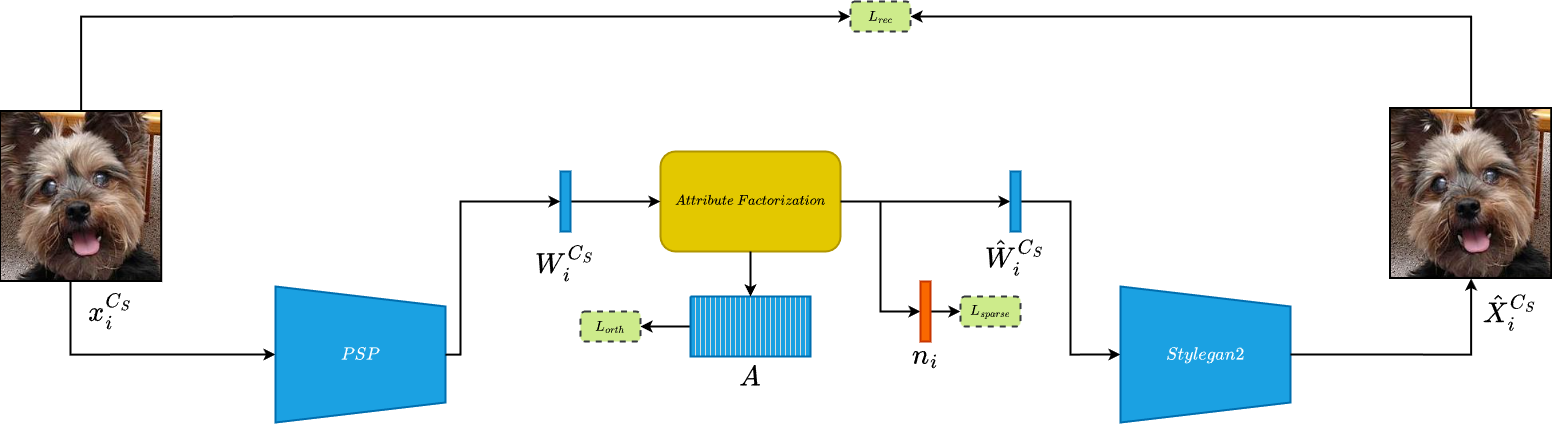
\includegraphics[width=1\linewidth]{images/SFSAGE.drawio.png}
    \caption{\textit{Attribute Factorization Training Framework \citep{ding2023stableattributegroupediting}}}
    \label{fig:attributge_fac_training}
\end{figure}

To enable disentangled editing, FeatureSAGE retains the SAGE attribute factorization block. The block learns category-irrelevant directions by comparing the latent code of a sample with the mean latent code of its category. The class embedding for a category is computed as the mean of its latent codes, as shown in Equation~\ref{eq:class-embedding}:

\begin{equation}
e^{C} = \frac{1}{N_C}\sum_{i=1}^{N_C} w_i^{C},
\label{eq:class-embedding}
\end{equation}

where $e^{C}$ is the class embedding for category $C$, $N_C$ is the number of latent codes available for the category, and $w_i^{C}$ is the latent code of the $i$th image. Equation~\ref{eq:class-embedding} provides the category-relevant center used to separate identity or class-level information from editable appearance variation.

\begin{figure}[ht]
    \centering
    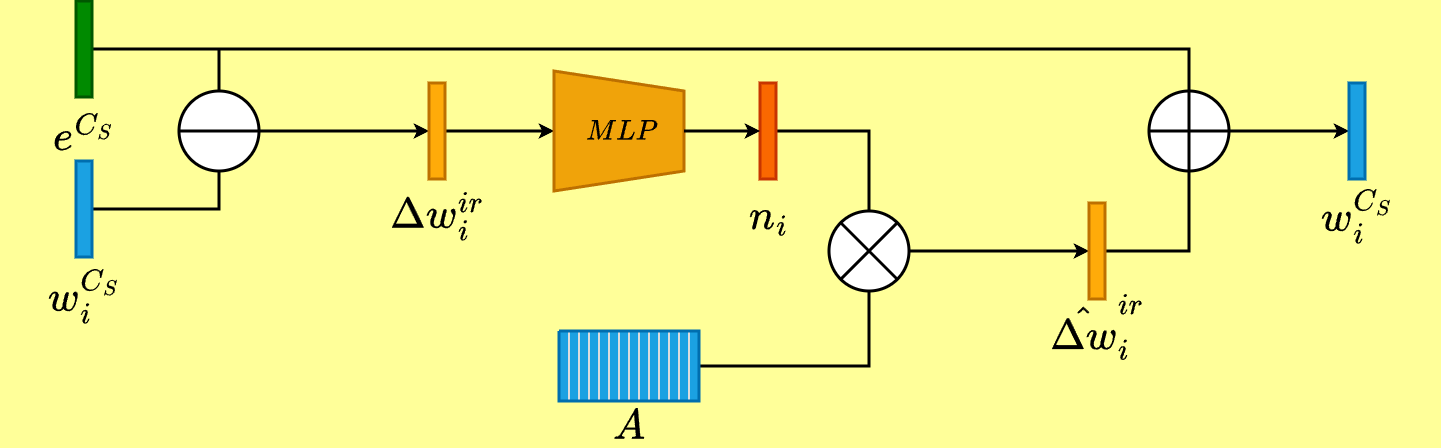
\includegraphics[width=1\linewidth]{images/AttributeFac.drawio.png}
    \caption{\textit{Attribute Factorization Block, derived from \citep{ding2023stableattributegroupediting}}}
    \label{fig:attribute_factorization_block}
\end{figure}

In the Attribute Factorization block shown in Figure~\ref{fig:attribute_factorization_block}, the category-irrelevant residual is computed in Equation~\ref{eq:category-irrelevant-residual}:

\begin{equation}
\Delta w_i^{ir}=w_i^{C_s}-e^{C_s}.
\label{eq:category-irrelevant-residual}
\end{equation}

In Equation~\ref{eq:category-irrelevant-residual}, $\Delta w_i^{ir}$ is the latent residual that remains after subtracting the class embedding $e^{C_s}$ from the sample latent code $w_i^{C_s}$. The purpose of this residual is to isolate appearance attributes that affect how an object looks without changing its class membership, such as orientation, color, background, texture, and expression.

The residual is then reconstructed using a learned sparse dictionary, as shown in Equation~\ref{eq:residual-factorization}:

\begin{equation}
\hat{\Delta w}_i^{ir}=A n_i.
\label{eq:residual-factorization}
\end{equation}

In Equation~\ref{eq:residual-factorization}, $A$ is the global dictionary of category-irrelevant directions and $n_i$ is the sparse coefficient vector predicted for the image. The dictionary basis follows sparse dictionary learning: each image is represented using only a small number of active directions so that individual directions remain more semantically interpretable.

Category-irrelevant editing is defined in Equation~\ref{eq:category-irrelevant-edit}. The edit changes appearance while preserving the category:

\begin{equation}
edit_{ir}(G(W_i^{C_s}))=
G\left(W_i^{C_s}+\alpha\Delta W^{ir},\,H(F_{k,i},\alpha\Delta W^{ir})\right)=\hat{X}_i^{C_s}.
\label{eq:category-irrelevant-edit}
\end{equation}

In Equation~\ref{eq:category-irrelevant-edit}, $edit_{ir}(\cdot)$ denotes category-irrelevant editing, $\alpha$ controls the edit intensity, $\Delta W^{ir}$ is the category-irrelevant direction, $H(\cdot)$ is the Feature Editor, and $\hat{X}_i^{C_s}$ is the edited image. The theoretical basis is the SAGE assumption that category-irrelevant directions can be learned from seen categories and transferred to unseen categories.

The sparse dictionary learning objective is stated in Equation~\ref{eq:sparse-dictionary-learning}:

\begin{equation}
\min_{n_i}\|n_i\|_0 \quad \mathrm{s.t.}\quad \Delta W_i^{ir}=A n_i.
\label{eq:sparse-dictionary-learning}
\end{equation}

In Equation~\ref{eq:sparse-dictionary-learning}, $\|n_i\|_0$ counts the number of nonzero entries in $n_i$. The purpose of the $L_0$ constraint is to encourage sparse use of the dictionary so that each generated edit is controlled by a limited number of directions.

In practice, SAGE optimizes this factorization with an encoder-decoder structure in which a Multi-Layer Perceptron (MLP) predicts the sparse representation, as shown in Equation~\ref{eq:mlp-sparse-code}:

\begin{equation}
n_i = MLP(\Delta W_i^{ir}).
\label{eq:mlp-sparse-code}
\end{equation}

Equation~\ref{eq:mlp-sparse-code} defines how the residual latent vector is encoded into the sparse coefficient vector used by the dictionary $A$.

% ======================================================================================================

\subsection{Class Embedding Mapping}

\begin{figure}[ht]
    \centering
    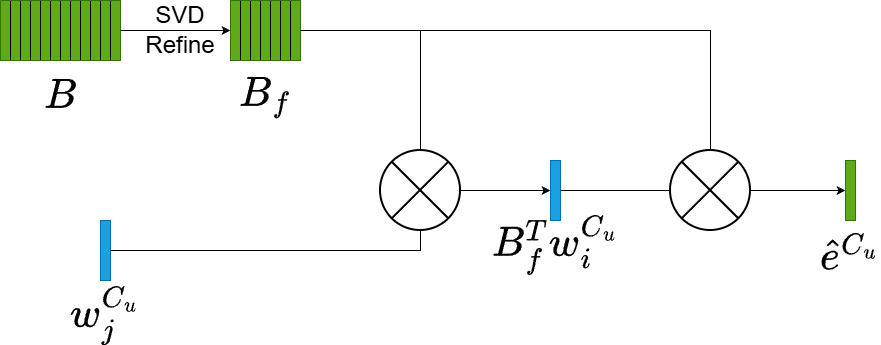
\includegraphics[width=1\linewidth]{images/Class_embedding_mapping.drawio.png}
    \caption{\textit{Class Embedding Block, adapted from \citep{ding2023stableattributegroupediting}}}
    \label{fig:class_embedding_block}
\end{figure}

Compared with Attribute Group Editing (AGE) \citep{AGE}, which randomly samples editing directions from $A$, SAGE uses class embedding mapping. The class embedding mapping block shown in Figure~\ref{fig:class_embedding_block} identifies the most important directions in the latent-code space for each category group and uses those directions to guide subsequent edits. This part of the framework remains unchanged in FeatureSAGE.

The class embedding set for the seen categories is denoted as $B$. Since the embeddings are computed from average latent codes, $B$ may still contain interference from category-irrelevant attributes. To filter the category-relevant subspace, singular value decomposition (SVD) is applied as shown in Equation~\ref{eq:svd-class-embedding}:

\begin{equation}
B = U_B \Sigma_B V_B^{T}.
\label{eq:svd-class-embedding}
\end{equation}

In Equation~\ref{eq:svd-class-embedding}, $B$ is the matrix of category-relevant class embeddings, $U_B$ contains the left singular vectors, $\Sigma_B$ contains singular values in descending order, and $V_B^{T}$ is the transpose of the right singular-vector matrix. The top-$t_B$ directions in $U_B$ are selected as the final category-relevant attribute dictionary $B_f \in \mathbb{R}^{18\times512\times t_B}$.

The class embedding of an unseen category is estimated using the filtered dictionary, as shown in Equation~\ref{eq:unseen-class-embedding}:

\begin{equation}
\hat{e}^{C_u} = \frac{1}{N_u}\sum_{i=1}^{N_u} B_f B_f^T W_i^{C_u}.
\label{eq:unseen-class-embedding}
\end{equation}

In Equation~\ref{eq:unseen-class-embedding}, $\hat{e}^{C_u}$ is the estimated embedding for unseen category $C_u$, $N_u$ is the number of latent codes available for that unseen category, and $W_i^{C_u}$ is the latent code of the $i$th unseen-category sample. The projection $B_fB_f^T W_i^{C_u}$ retains category-relevant components while suppressing most category-irrelevant variation.

% ======================================================================================================

\subsection{Adaptive Editing}

\begin{figure}[ht]
    \centering
    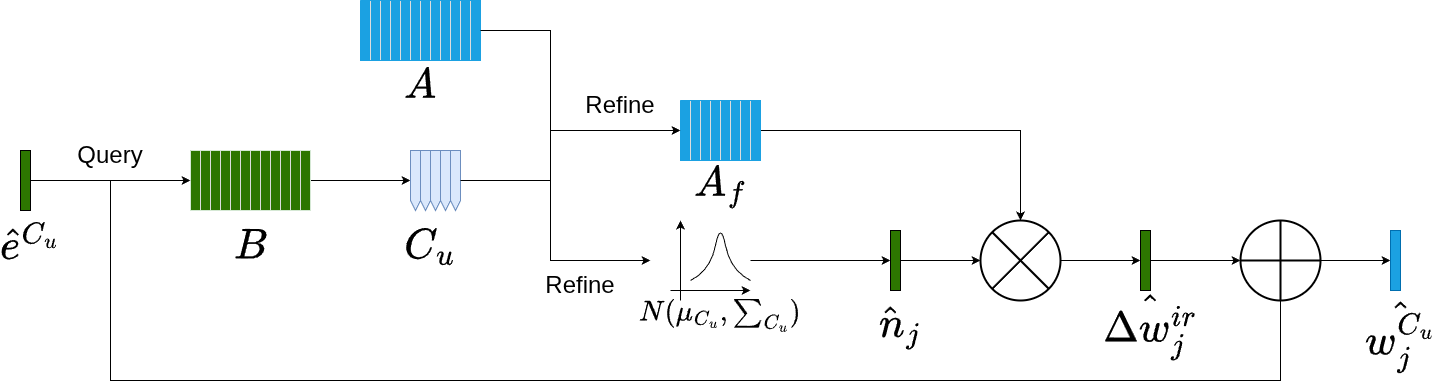
\includegraphics[width=1\linewidth]{images/adaptive.drawio.png}
    \caption{\textit{Adaptive Editing Block, from \citep{ding2023stableattributegroupediting}}}
    \label{fig:adaptive_editing_block}
\end{figure}

Figure~\ref{fig:adaptive_editing_block} shows the adaptive editing block of FeatureSAGE. Category-irrelevant qualities typically have similar distributions in closely related categories but may differ across distant categories. Therefore, adaptive editing selects seen categories that are close to an unseen category in the class-embedding space and uses their common editing directions to guide generation.

To identify the category-irrelevant editing directions that best fit an unseen category $C_u$, the residual direction is back-projected into the sparse representation, as shown in Equation~\ref{eq:back-projection}:

\begin{equation}
\hat{n}_i = A^{\dagger}\Delta W_i^{ir}.
\label{eq:back-projection}
\end{equation}

In Equation~\ref{eq:back-projection}, $A^{\dagger}$ denotes the pseudo-inverse of the dictionary $A$, $\Delta W_i^{ir}$ is the category-irrelevant residual, and $\hat{n}_i$ is the estimated sparse representation. The pseudo-inverse is used to express an observed residual in the coordinate system of the learned dictionary.

The mean absolute activation of sparse directions across the top-$t_C$ similar seen categories is computed in Equation~\ref{eq:mean-absolute-sparse-code}:

\begin{equation}
\overline{|n|}^{C_u} =
\frac{1}{t_C}\sum_{t=1}^{t_C}
\frac{1}{N_{S_t}}\sum_{i=1}^{N_{S_t}}
\left|\hat{n}_i^{C_{S_t}}\right|.
\label{eq:mean-absolute-sparse-code}
\end{equation}

In Equation~\ref{eq:mean-absolute-sparse-code}, $t_C$ is the number of similar seen categories, $N_{S_t}$ is the number of samples in the $t$th selected seen category, and $\hat{n}_i^{C_{S_t}}$ is the sparse representation of the $i$th sample from that category. The result $\overline{|n|}^{C_u}$ measures which dictionary directions are frequently or strongly activated for categories similar to $C_u$. For each layer in $W^+$, the top-$t_A$ directions are selected from $A$ to form the adaptive category-irrelevant dictionary $A_{C_u}\in\mathbb{R}^{18\times512\times t_A}$.

SAGE assumes that the sparse representations for related categories follow a Gaussian distribution. This distribution is estimated in Equation~\ref{eq:adaptive-gaussian}:

\begin{equation}
\tilde{n}_j \sim \mathcal{N}(\mu_{C_u},\Sigma_{C_u}).
\label{eq:adaptive-gaussian}
\end{equation}

In Equation~\ref{eq:adaptive-gaussian}, $\mu_{C_u}$ and $\Sigma_{C_u}$ are the estimated mean and covariance of sparse codes for the selected categories, and $\tilde{n}_j$ is a sampled sparse code used to generate a new image. This sampling step provides controlled diversity for the unseen category.

The final adaptive generation equation is given in Equation~\ref{eq:adaptive-generation}:

\begin{equation}
X_j^{C_u} =
G\left(\hat{e}^{C_u}+\alpha A_{C_u}\tilde{n}_j,\,
H(F_{k,j}^{C_u},\alpha A_{C_u}\tilde{n}_j)\right).
\label{eq:adaptive-generation}
\end{equation}

In Equation~\ref{eq:adaptive-generation}, $X_j^{C_u}$ is a generated image for unseen category $C_u$, $\hat{e}^{C_u}$ is the estimated class embedding, $A_{C_u}$ is the adaptive dictionary, $\tilde{n}_j$ is the sampled sparse code, $\alpha$ controls the strength of the edit, and $H(\cdot)$ edits the feature tensor used by the generator. This equation summarizes how FeatureSAGE transforms one-shot class information and sampled attribute variation into a generated image.

% ======================================================================================================

\subsection{Feature Editing Decoder Block}

\begin{figure}[ht]
    \centering
    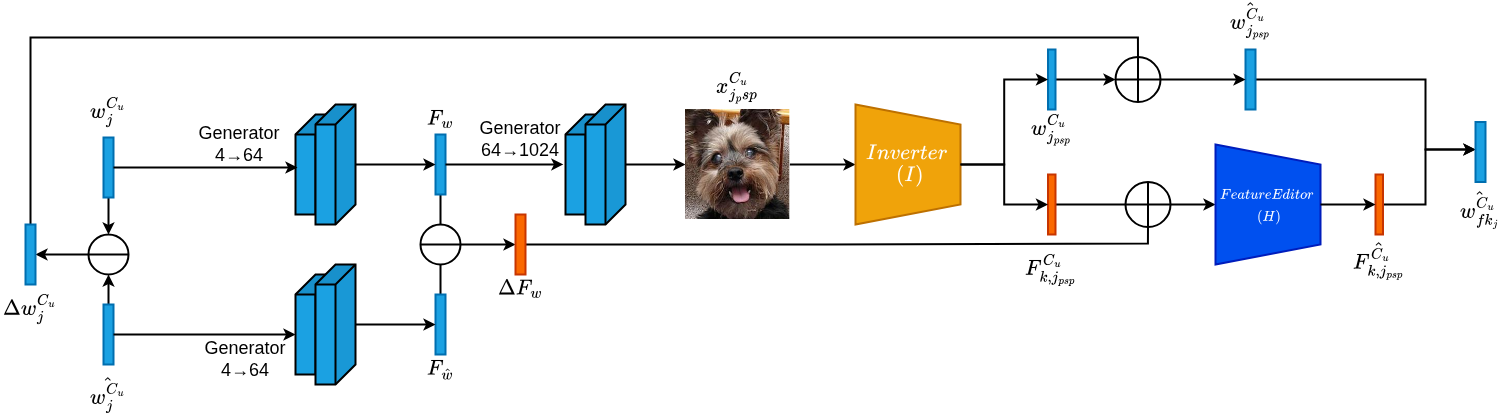
\includegraphics[width=1\linewidth]{images/featureEditordrawio.drawio.png}
    \caption{\textit{Feature Editing Decoder Block}}
    \label{fig:featureEditingBlock}
\end{figure}

Figure~\ref{fig:featureEditingBlock} shows the Feature Editing Decoder Block. The block receives the original latent representation, the edited latent representation produced by adaptive editing, and the intermediate feature tensor extracted by the StyleFeatureEditor inverter. Its role is to transform the input features into an edited feature tensor that can be injected into the ninth StyleGAN feature layer during image synthesis.

The latent-space difference used to describe the semantic edit is defined in Equation~\ref{eq:latent-difference}:

\begin{equation}
\Delta w_j^{C_u}=\hat{w}_j^{C_u}-w_j^{C_u}.
\label{eq:latent-difference}
\end{equation}

In Equation~\ref{eq:latent-difference}, $w_j^{C_u}$ is the original latent code and $\hat{w}_j^{C_u}$ is the edited latent code. This difference specifies the semantic movement applied in $W^+$.

The feature-space difference used for feature injection is defined in Equation~\ref{eq:feature-difference}:

\begin{equation}
\Delta F_w = F_w - F_{\hat{w}}.
\label{eq:feature-difference}
\end{equation}

In Equation~\ref{eq:feature-difference}, $F_w$ is the intermediate feature tensor produced from the original latent code and $F_{\hat{w}}$ is the corresponding tensor produced from the edited latent code. The decoder block uses this difference to determine how the original feature tensor should be modified to match the target semantic edit.

The Feature Editor transformation is represented in Equation~\ref{eq:feature-editor-transform}:

\begin{equation}
F_{k,j}^{\mathrm{edit}} = H(F_{k,j}^{C_u}, \Delta F_w).
\label{eq:feature-editor-transform}
\end{equation}

In Equation~\ref{eq:feature-editor-transform}, $F_{k,j}^{C_u}$ is the feature tensor extracted by the inverter for the unseen-category input, $\Delta F_w$ is the feature difference from Equation~\ref{eq:feature-difference}, and $F_{k,j}^{\mathrm{edit}}$ is the edited tensor injected into the generator. The decoder therefore modifies the feature-level representation while the edited latent code controls the global semantic direction. The output image is then synthesized by the generator using the edited latent code and the edited feature tensor, as shown in Equation~\ref{eq:decoder-synthesis}:

\begin{equation}
\hat{X}_j^{C_u}=G(\hat{w}_j^{C_u}, F_{k,j}^{\mathrm{edit}}).
\label{eq:decoder-synthesis}
\end{equation}

Equation~\ref{eq:decoder-synthesis} completes the decoder pathway: input image features and latent edits are transformed into an edited high-resolution output.

% ======================================================================================================
\subsection{Training Strategy}

In the training stage, a StyleGAN2 generator is trained using images from the seen categories. The StyleFeatureEditor inverter and the pSp encoder are also trained or used according to their roles in the pipeline. To manage resource consumption, FeatureSAGE uses a two-phase strategy: attribute factorization training followed by Feature Editor training.

\subsection{Phase 1: Attribute Factorization Training}

Phase 1 trains the attribute factorization block for disentangled sampling of category-irrelevant directions. The following losses are applied to the attribute factorization block.

\begin{itemize}
    \item \textbf{Sparsity Loss ($L_{\mathrm{sparse}}$):} The sparsity loss encourages the learned attribute code to activate only a small number of dictionary directions. Equation~\ref{eq:sparsity-loss} defines the loss:
    \begin{equation}
    L_{\mathrm{sparse}} = \left\|\sigma(\theta_0 n_i-\theta_1)\right\|_1.
    \label{eq:sparsity-loss}
    \end{equation}
    In Equation~\ref{eq:sparsity-loss}, $\sigma(\cdot)$ denotes the sigmoid function, $n_i$ is the sparse code, and $\theta_0$ and $\theta_1$ are hyperparameters controlling sparsity. The sigmoid compresses the MLP output and the $L_1$ norm approximates sparse behavior in a differentiable way.

    \item \textbf{Reconstruction Loss ($L_{\mathrm{rec}}$):} The reconstruction loss anchors the edited output to the input image so that edits do not destroy the original content. Equation~\ref{eq:reconstruction-loss} defines this loss:
    \begin{equation}
    L_{\mathrm{rec}}=\left\|G(e^{C_s}+A n_i)-x_i^{C_s}\right\|_2.
    \label{eq:reconstruction-loss}
    \end{equation}
    In Equation~\ref{eq:reconstruction-loss}, $e^{C_s}$ is the class-center latent, $A n_i$ is the attribute offset, $G(\cdot)$ is the generator, and $x_i^{C_s}$ is the input image. The loss penalizes large differences between the generated reconstruction and the original image.

    \item \textbf{Orthogonality Loss ($L_{\mathrm{orth}}$):} The orthogonality loss discourages category-irrelevant directions from overlapping with category-relevant directions. Equation~\ref{eq:orthogonality-loss} defines this loss:
    \begin{equation}
    L_{\mathrm{orth}}=\left\|B^T A\right\|_F^2.
    \label{eq:orthogonality-loss}
    \end{equation}
    In Equation~\ref{eq:orthogonality-loss}, $A$ is the category-irrelevant dictionary, $B$ is the category-relevant embedding basis, and $\|\cdot\|_F^2$ denotes the squared Frobenius norm. This term preserves class identity by reducing leakage between the category-relevant and category-irrelevant subspaces.
\end{itemize}

The overall attribute factorization loss is defined in Equation~\ref{eq:attribute-factorization-loss}:

\begin{equation}
L_{\mathrm{af}}=L_{\mathrm{rec}}+\lambda_1 L_{\mathrm{orth}}+\lambda_2 L_{\mathrm{sparse}}.
\label{eq:attribute-factorization-loss}
\end{equation}

In Equation~\ref{eq:attribute-factorization-loss}, $\lambda_1$ and $\lambda_2$ are weights for the orthogonality and sparsity losses \citep{ding2023stableattributegroupediting}. Training uses the Adam optimizer with a fixed learning rate of $1\times10^{-4}$, $\lambda_1=5\times10^{-4}$, $\lambda_2=5\times10^{-3}$, $\theta_0=5\times10^{-1}$, and $\theta_1=-1$.

\subsection{Phase 2: Feature Editor Training}

Phase 2 trains the Feature Editor $H$ using editing pairs generated with a pretrained pSp encoder. Following \citet{bobkov2024devildetailsstylefeatureeditordetailrich}, an input image $X$ is encoded into $w$, edited by a sampled direction from the adaptive editing procedure, and paired with the corresponding edited image $\hat{X}$. This trains $H$ to edit feature tensors according to the category-irrelevant attributes learned in Phase 1. To prevent the Feature Editor from relying only on synthetic editing pairs, it is also trained on the classical inversion task with $\Delta=0$.

The editing loss is defined in Equation~\ref{eq:feature-edit-loss}:

\begin{equation}
L_{\mathrm{edit}}(X,\hat{X}) =
\lambda_{l_2}\|X-\hat{X}\|_2+
\lambda_{\mathrm{lpips}}\mathcal{L}_{\mathrm{lpips}}(X,\hat{X}).
\label{eq:feature-edit-loss}
\end{equation}

The inversion loss uses the same reconstruction and perceptual terms, as shown in Equation~\ref{eq:feature-inversion-loss}:

\begin{equation}
L_{\mathrm{inv}}(X,\hat{X}) =
\lambda_{l_2}\|X-\hat{X}\|_2+
\lambda_{\mathrm{lpips}}\mathcal{L}_{\mathrm{lpips}}(X,\hat{X}).
\label{eq:feature-inversion-loss}
\end{equation}

Equations~\ref{eq:feature-edit-loss} and \ref{eq:feature-inversion-loss} use $L_2$ reconstruction and LPIPS perceptual losses to preserve both pixel-level structure and perceptual similarity. The total Feature Editor loss is defined in Equation~\ref{eq:feature-editor-loss}:

\begin{equation}
L_{\mathrm{fe}} = L_{\mathrm{edit}}(X,\hat{X}) + L_{\mathrm{inv}}(X,\hat{X}).
\label{eq:feature-editor-loss}
\end{equation}

In Equation~\ref{eq:feature-editor-loss}, the editing term teaches $H$ to respond to nonzero edit directions, while the inversion term with $\Delta=0$ stabilizes feature reconstruction. The Feature Editor is trained using the Adam optimizer with a fixed learning rate of $1\times10^{-4}$ for 15,000 iterations on a single V100 16 GB vGPU. Mixed precision is enabled to improve memory efficiency because the phase requires multiple generator passes. The loss weights are $\lambda_{l_2}=10$ and $\lambda_{\mathrm{lpips}}=0.8$, with an additional LPIPS scaling factor of 0.5. The sparse dictionary $A$ is initialized with a fixed length of 100.
